\documentclass{article}
% 夾帶 fixture 共用的樣式：只用 TikZ 內建與常見函式庫，字為 ASCII，不需要 CJK 字型。
\usepackage{tikz}
\usetikzlibrary{arrows.meta,positioning,fit,backgrounds,shapes.geometric,calc}
\tikzset{
  box/.style={rectangle, rounded corners=3pt, draw, fill=blue!8, minimum height=8mm, minimum width=22mm, align=center},
  decision/.style={diamond, aspect=2.4, draw, fill=gray!8, align=center, inner sep=2pt},
  flow/.style={-{Stealth[length=2.5mm]}, thick},
  lab/.style={font=\scriptsize, fill=white, inner sep=2pt},
  annot/.style={rectangle, draw, dashed, fill=white, font=\footnotesize, align=center},
  leader/.style={densely dotted, shorten >=2pt, shorten <=2pt},
  region/.style={draw, dashed, rounded corners=4pt, fill=gray!6, inner sep=8pt},
}

\begin{document}

% 流程圖：外框（fit）、外框內的標題字、從外面接進外框成員的線、
% 註記與 leader 虛線、壓在自己線上的白底標籤、菱形、轉折線與傾斜標籤。
% expect: none
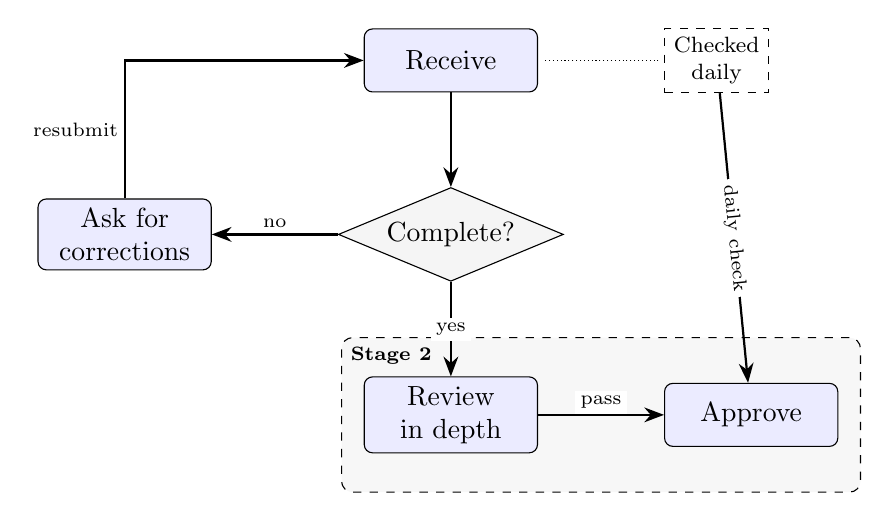
\begin{tikzpicture}[node distance=12mm and 16mm]
  \node[box] (start) {Receive};
  \node[decision, below=of start] (ok) {Complete?};
  \node[box, below=of ok] (review) {Review\\in depth};
  \node[box, left=of ok] (fix) {Ask for\\corrections};
  \node[box, right=of review] (done) {Approve};
  \node[annot, right=of start] (note) {Checked\\daily};
  \begin{scope}[on background layer]
    \node[region, fit=(review)(done), inner ysep=14pt] (stage) {};
  \end{scope}
  \node[font=\scriptsize\bfseries, anchor=north west] at (stage.north west) {Stage 2};
  \draw[flow] (start) -- (ok);
  \draw[flow] (ok) -- node[lab] {yes} (review);
  \draw[flow] (ok) -- node[lab, above] {no} (fix);
  \draw[flow] (fix) |- node[lab, pos=0.25, left] {resubmit} (start);
  \draw[flow] (review) -- node[lab, above] {pass} (done);
  \draw[leader] (note) -- (start);
  \draw[flow] (note) -- node[lab, sloped] {daily check} (done);
\end{tikzpicture}

% 同一接點分岔與匯流（共用線段是刻意的）、預設的 -> 箭頭、double 線、無框的節點旁註。
% expect: none
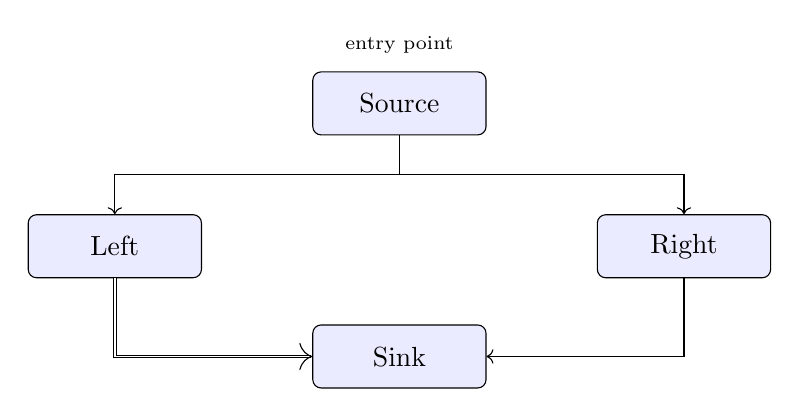
\begin{tikzpicture}[node distance=10mm and 14mm]
  \node[box] (src) {Source};
  \node[box, below left=of src] (l) {Left};
  \node[box, below right=of src] (r) {Right};
  \node[box, below=24mm of src] (sink) {Sink};
  \draw[->] (src.south) -- ++(0,-5mm) -| (l.north);
  \draw[->] (src.south) -- ++(0,-5mm) -| (r.north);
  \draw[->, double] (l.south) |- (sink.west);
  \draw[->] (r.south) |- (sink.east);
  \node[font=\scriptsize, above=1mm of src] {entry point};
\end{tikzpicture}

\end{document}
